\documentclass{article}
\usepackage[utf8]{inputenc}

\title{\textbf{Optimal low-thrust navigation around bilobate asteroids with sequential convex programming}}
\author{Rory Lipkis, \textit{Stanford University, Department of Aeronautics and Astronautics}}
\date{}
\newcommand{\uvec}[1]{\boldsymbol{\hat{\textbf{#1}}}}
\newcommand{\conj}[1]{{#1}^{\dagger}}
\newcommand{\del}{\nabla}
\newcommand{\D}{\mathrm{d}}
\newcommand{\TD}[2]{\frac{d#1}{d#2}}
\newcommand{\TTD}[2]{\frac{d^{2}{#1}}{d{#2}^{2}}}
\newcommand{\PD}[2]{\frac{\partial#1}{\partial#2}}
\newcommand{\PPD}[2]{\frac{\partial^{2}{#1}}{\partial{#2}^{2}}}
\newcommand{\PPPD}[2]{\frac{\partial^{3}{#1}}{\partial{#2}^{3}}}
\newcommand{\la}{\langle}
\newcommand{\ra}{\rangle}
\newcommand{\const}[1]{\Big\rvert_{#1}}
\newcommand{\pfrac}[2]{\left(\frac{#1}{#2}\right)}
\usepackage{fullpage}
\usepackage{amsmath}
\usepackage{amssymb}
\usepackage{setspace}
\usepackage{mathtools}
\usepackage{enumerate}
\usepackage{esint}
\usepackage{booktabs}
\usepackage{physics}
\usepackage{siunitx}
\usepackage{graphicx}
\usepackage{graphics}
\usepackage{dsfont}
\usepackage{slashed}
\usepackage{multicol}
\usepackage{float}

\begin{document}

\maketitle

\begin{multicols}{2}
\section*{Introduction}
As interest in asteroid exploration missions increases, there is potential use for low-thrust control around irregularly-shaped gravitating bodies. Recent missions to asteroids 67P/Churyumov–Gerasimenko (Rosetta) and 486958 Arrokoth (New Horizons) revealed bilobate shapes, which appear to be a relatively common feature of asteroids (see Figure \ref{fig:67P}). These shapes, also known as \textit{contact binaries}, produce highly nonspherical gravitational potentials that cannot be easily navigated. 

Stacey and D'Amico 2018\footnote{Stacey, Nathan, and Simone D’Amico. ``Autonomous Swarming for Simultaneous Navigation and Asteroid Characterization.'' In \emph{AAS/AIAA Astrodynamics Specialist Conference}. 2018.} describe a method by which satellite formations could be used to perform initial estimation of asteroid gravitational fields. Although such gravitational fields must necessarily be very weak (or else the bodies would be pulled into spheroid), future missions that entail a large number of asteroid visits or independent spacecrafts must contend with potentially stringent thrust constraints, which limit the spacecraft control ability to within an order of magnitude of the surface gravity. In this domain, the irregularity of the gravitational becomes a nontrivial consideration.

Irregular gravitational fields are typically represented by their decomposition into spherical harmonics, the basis of Legendre polynomials. The standard orbital element representation of orbital motion can be modified to account for low-order harmonics, such as the $J2$ oblateness correction, with the introduction of mean and osculating elements, which specify an ``instantaneous'' unperturbed orbit. This extension allows control schemes that rely on orbital elements to be easily extended to find optimal thrust solutions around slightly oblate bodies. Though useful for orbits around planets, this method does not generalize to trajectories in highly irregular gravitational fields, whose specifications require extremely high order spherical harmonics, and where the notion of orbital elements ceases to be meaningful altogether. Since such trajectories are rarely stable orbits, and in fact are nearly always chaotic, they cannot be meaningfully specified by any set of periodic elements, and the Cartesian position and velocity state must be used instead.

\begin{figure}[H]
	\centering
	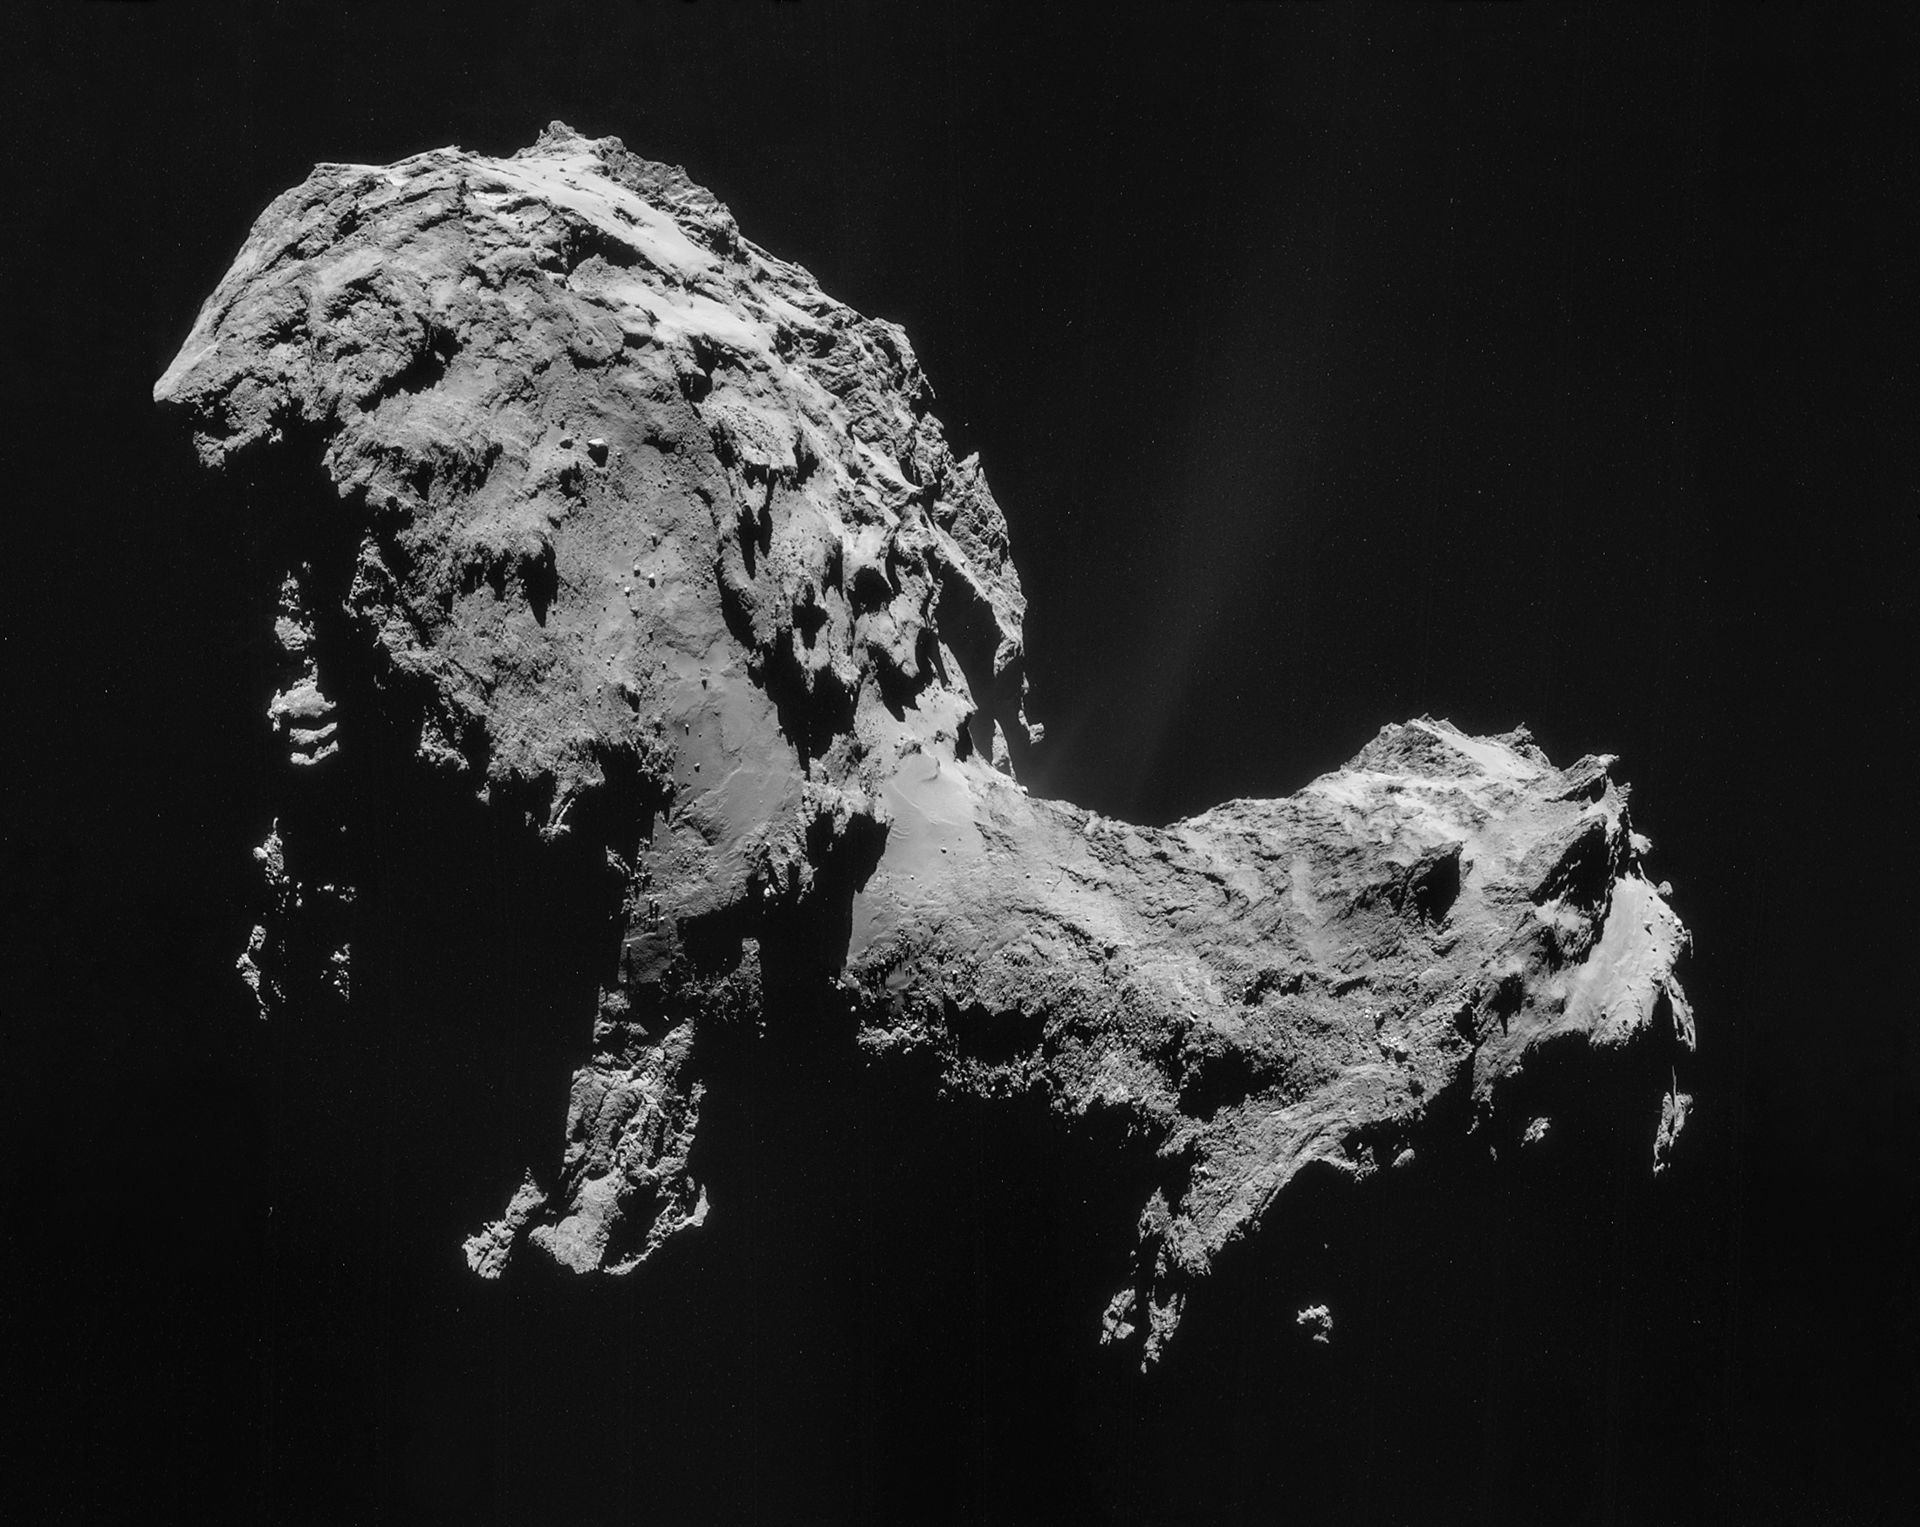
\includegraphics[width=0.8\linewidth]{comet}
	\caption{Comet 67P, \textit{via Wikipedia}.}
	\label{fig:67P}
\end{figure}

\section*{Asteroid model}
This paper examines a simplified model of a bilobate asteroid, consisting of two spherical masses of constant density, each with radius $R_{i}$, oriented along an axis $\uvec{a}$. By modeling the asteroid in this way, the costly spherical harmonic representation is replaced by a direct Newtonian calculation, which allows for much higher ``orders'' to be effectively considered, despite the reduced detail. The graviational field of the asteroid is then given by
\begin{align*}
	\mathbf{f}_{g} = -\frac{GM_{1}(\mathbf{r} - \mathbf{r}_{1})}{|\mathbf{r} - \mathbf{r}_{1}|^{3}} - \frac{GM_{2}(\mathbf{r} - \mathbf{r}_{2})}{|\mathbf{r} - \mathbf{r}_{2}|^{3}}
\end{align*}
where
\begin{align*}
	\mathbf{r}_{1} &= \frac{m_{2}}{m_{1} + m_{2}}(R_{1} + R_{2})\uvec{a}\\
	\mathbf{r}_{2} &= -\frac{m_{1}}{m_{1} + m_{2}}(R_{1} + R_{2})\uvec{a}
\end{align*}
are the positions of the lobe centers in the center-of-mass frame.

\section*{Sequential convex programming}
The system is formalized by the state $\mathbf{s}$, formed by the concatenation of the spacecraft position and velocity. Along with the control input $\mathbf{u}$, the dynamics are written as
\begin{align*}
	\dot{\mathbf{s}} = \mathbf{f}(\mathbf{s}, \mathbf{u}) = 
	\begin{bmatrix}
	\mathbf{v}\\
	\mathbf{f}_{g} + \mathbf{u}
	\end{bmatrix}
\end{align*}
This is linearized around a reference state $\mathbf{s}_{0}$ and control input $\mathbf{u}_{0}$ by the first-order expansion
\begin{align*}
	\dot{\mathbf{s}} = \mathbf{f}(\mathbf{s}_{0}, \mathbf{u}_{0}) + A(\mathbf{s} - \mathbf{s}_{0}) + B(\mathbf{u} - \mathbf{u}_{0})
\end{align*}
The system matrix $A$ is given by
\begin{align*}
	A = \PD{\mathbf{f}}{\mathbf{s}}(\mathbf{s}_{0}, \mathbf{u}_{0}) =
	\begin{bmatrix}
	\mathbf{0}_{3\times3} & \mathbf{I}_{3\times3}\\
	A_{1} + A_{2} & \mathbf{0}_{3\times3}
	\end{bmatrix}
\end{align*}
where
\begin{align*}
	A_{i} = \frac{\mu(3\mathbf{d}_{i}\mathbf{d}_{i}^{T} - |\mathbf{d}_{i}|^{2}\mathbf{I}_{3\times3})}{|\mathbf{d}_{i}|^{5}}
\end{align*}
and $\mathbf{d}_{i} = \mathbf{r} - \mathbf{r}_{i}$ is the separation from a lobe center. The control matrix $B$ is given by
\begin{align*}
	B = \PD{\mathbf{f}}{\mathbf{u}}(\mathbf{s}_{0}, \mathbf{u}_{0}) = 
	\begin{bmatrix}
	\mathbf{0}_{3\times3}\\
	\mathbf{I}_{3\times3}
	\end{bmatrix}
\end{align*}
The sequential convex programming method solves at each iteration the problem
\begin{align*}
	\text{min} &\quad J(\mathbf{s}, \mathbf{u})\\
	\text{s.t.} &\quad \dot{\mathbf{s}}(t) = \mathbf{f}_{k}(\mathbf{s}(t), \mathbf{u}(t))\\
	&\quad \mathbf{s}(0) = \mathbf{s}_{0}\\
	&\quad \mathbf{u}(t) \in \mathcal{U}\\
	&\quad |\mathbf{s}(t) - \mathbf{s}_{k}(t)| \le \rho, \quad t \in [0,t_{f}]\\
\end{align*}
where $\mathbf{f}_{k}$ is the linearization of the dynamics with the previous solution trajectory $\mathbf{s}_{k}$ and control history $\mathbf{u}_{k}$ used as references. The dynamics constraint is enforced by a naive Euler integration that equates 
\begin{align*}
	\mathbf{s}_{t+1} = \mathbf{s}_{t} + \mathbf{f}_{k}(\mathbf{s}(t), \mathbf{u}(t))\Delta t
\end{align*}

% talk about modifications to cost, normalization, etc.
% show convergence plot

\section*{Implementation}
Several things must be noted:
\begin{enumerate}[(a)]
	\setlength{\itemsep}{0pt}
	\setlength{\parskip}{0pt}
	\item The equations of gravitational motion linearize notoriously poorly, and thus the trust region $\rho$ must be monitored closely.
	\item Neither the exact nor linearized dynamics admit a useful non-dimensional form. As a result, actual values for distance and mass must be used, which can result in extremely large costs that destabilize the convex solver. The cost matrices must be carefully scaled to produce a cost of a reasonable order of magnitude.
	\item Additionally, the cost is a function of the control history and the final state, but not the entire trajectory:
	\begin{align*}
		J(\mathbf{s}, \mathbf{u}) = \mathbf{s}(t_{f})^{T}Q_{f}\mathbf{s}(t_{f}) + \int_{0}^{t_{f}} \mathbf{u}(t)^{T}R\mathbf{u}(t)\,dt
	\end{align*}
	The large distances involved at the beginning of a regularization problem would otherwise result in large terms in the cost that completely overwhelmed the control terms.
\end{enumerate}

% poor linearization / sensitive convergence
% difficult to scale

\section*{Example mission}

\section*{}

\end{multicols}
\end{document}